\begin{frame}
    \frametitle{Arquitetura base - sem mecanismos de gestao de filas}
    \begin{figure}
        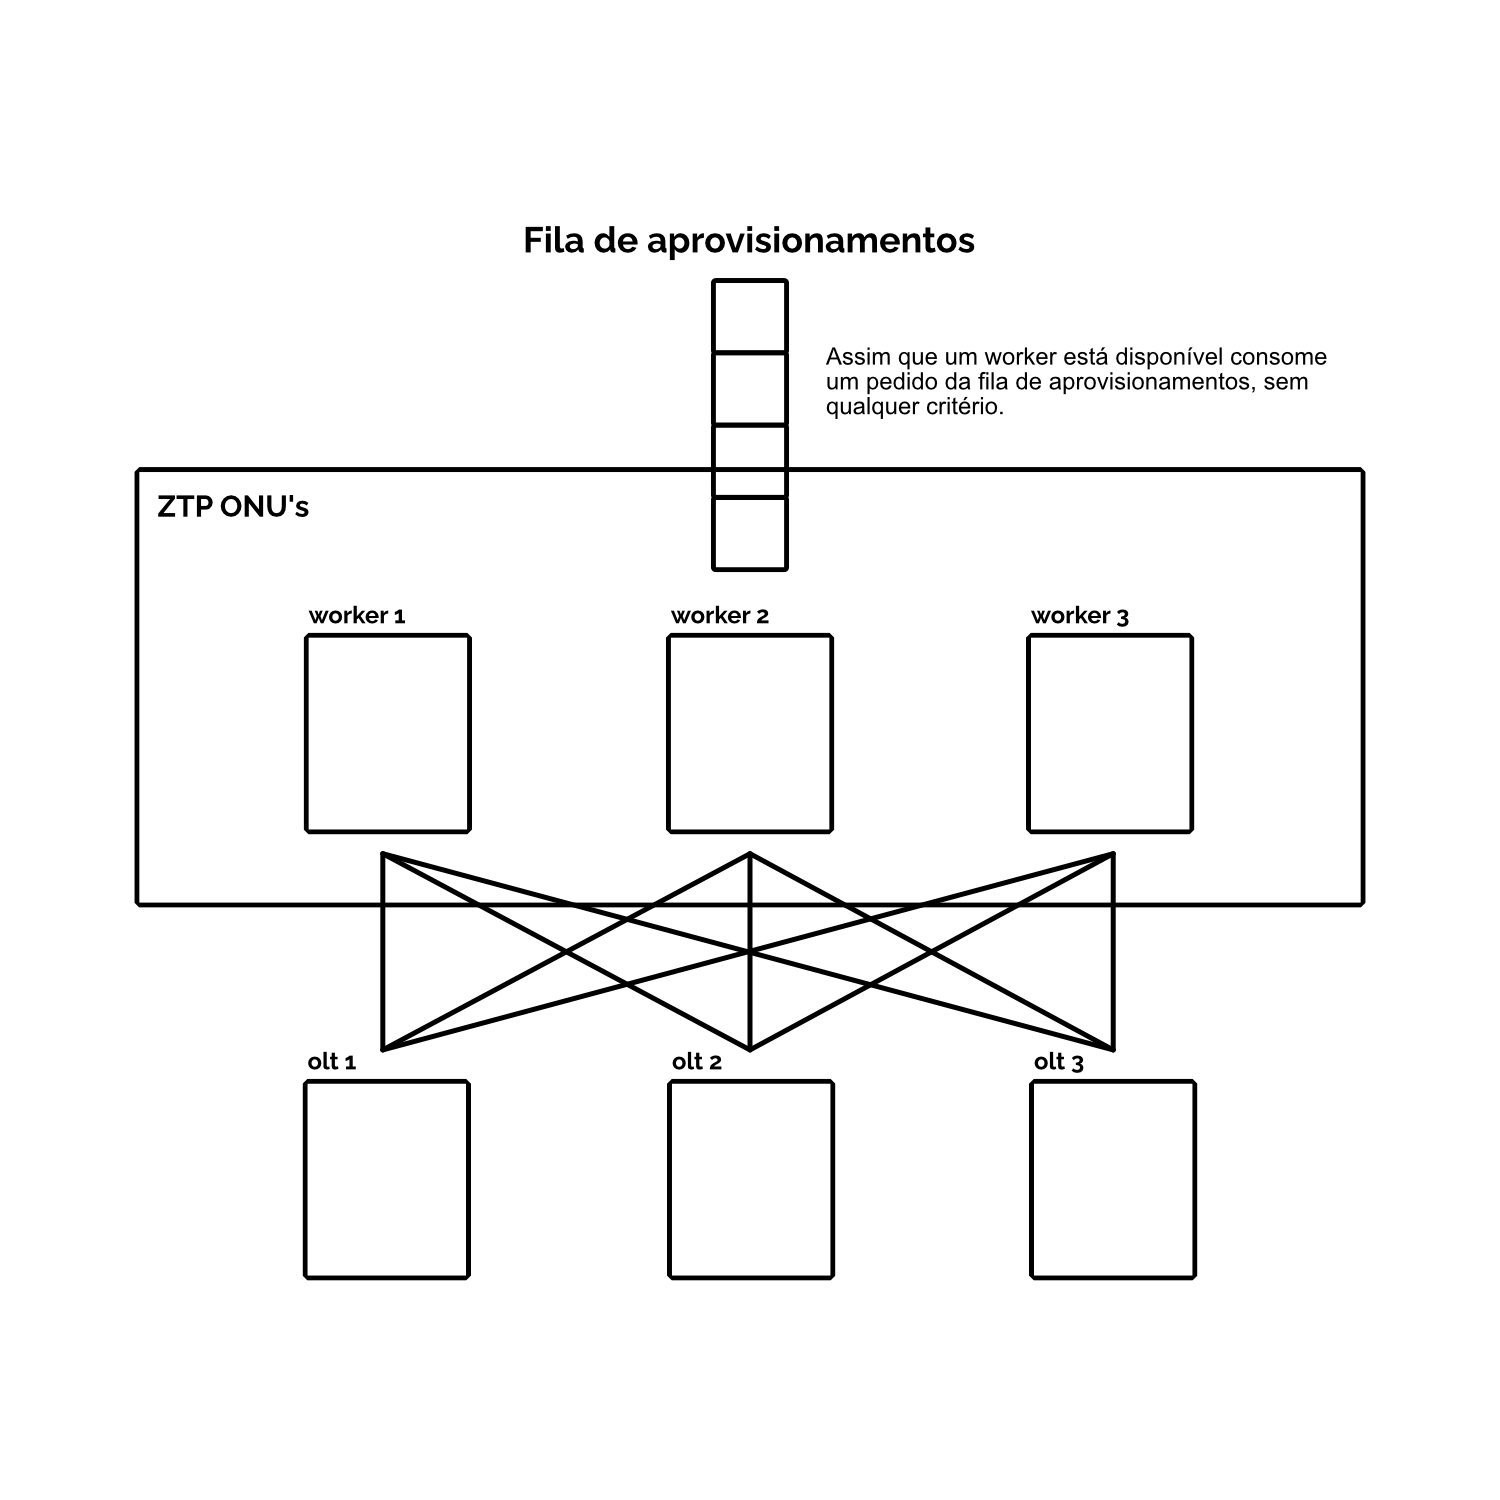
\includegraphics[width=0.8\textwidth]{./assets/gestao_de_filas/arquitetura_algoritmo_1.png}
    \end{figure}    
\end{frame}

\begin{frame}
    \frametitle{Arquitetura melhorada - 1ª alternativa}
    \begin{figure}
        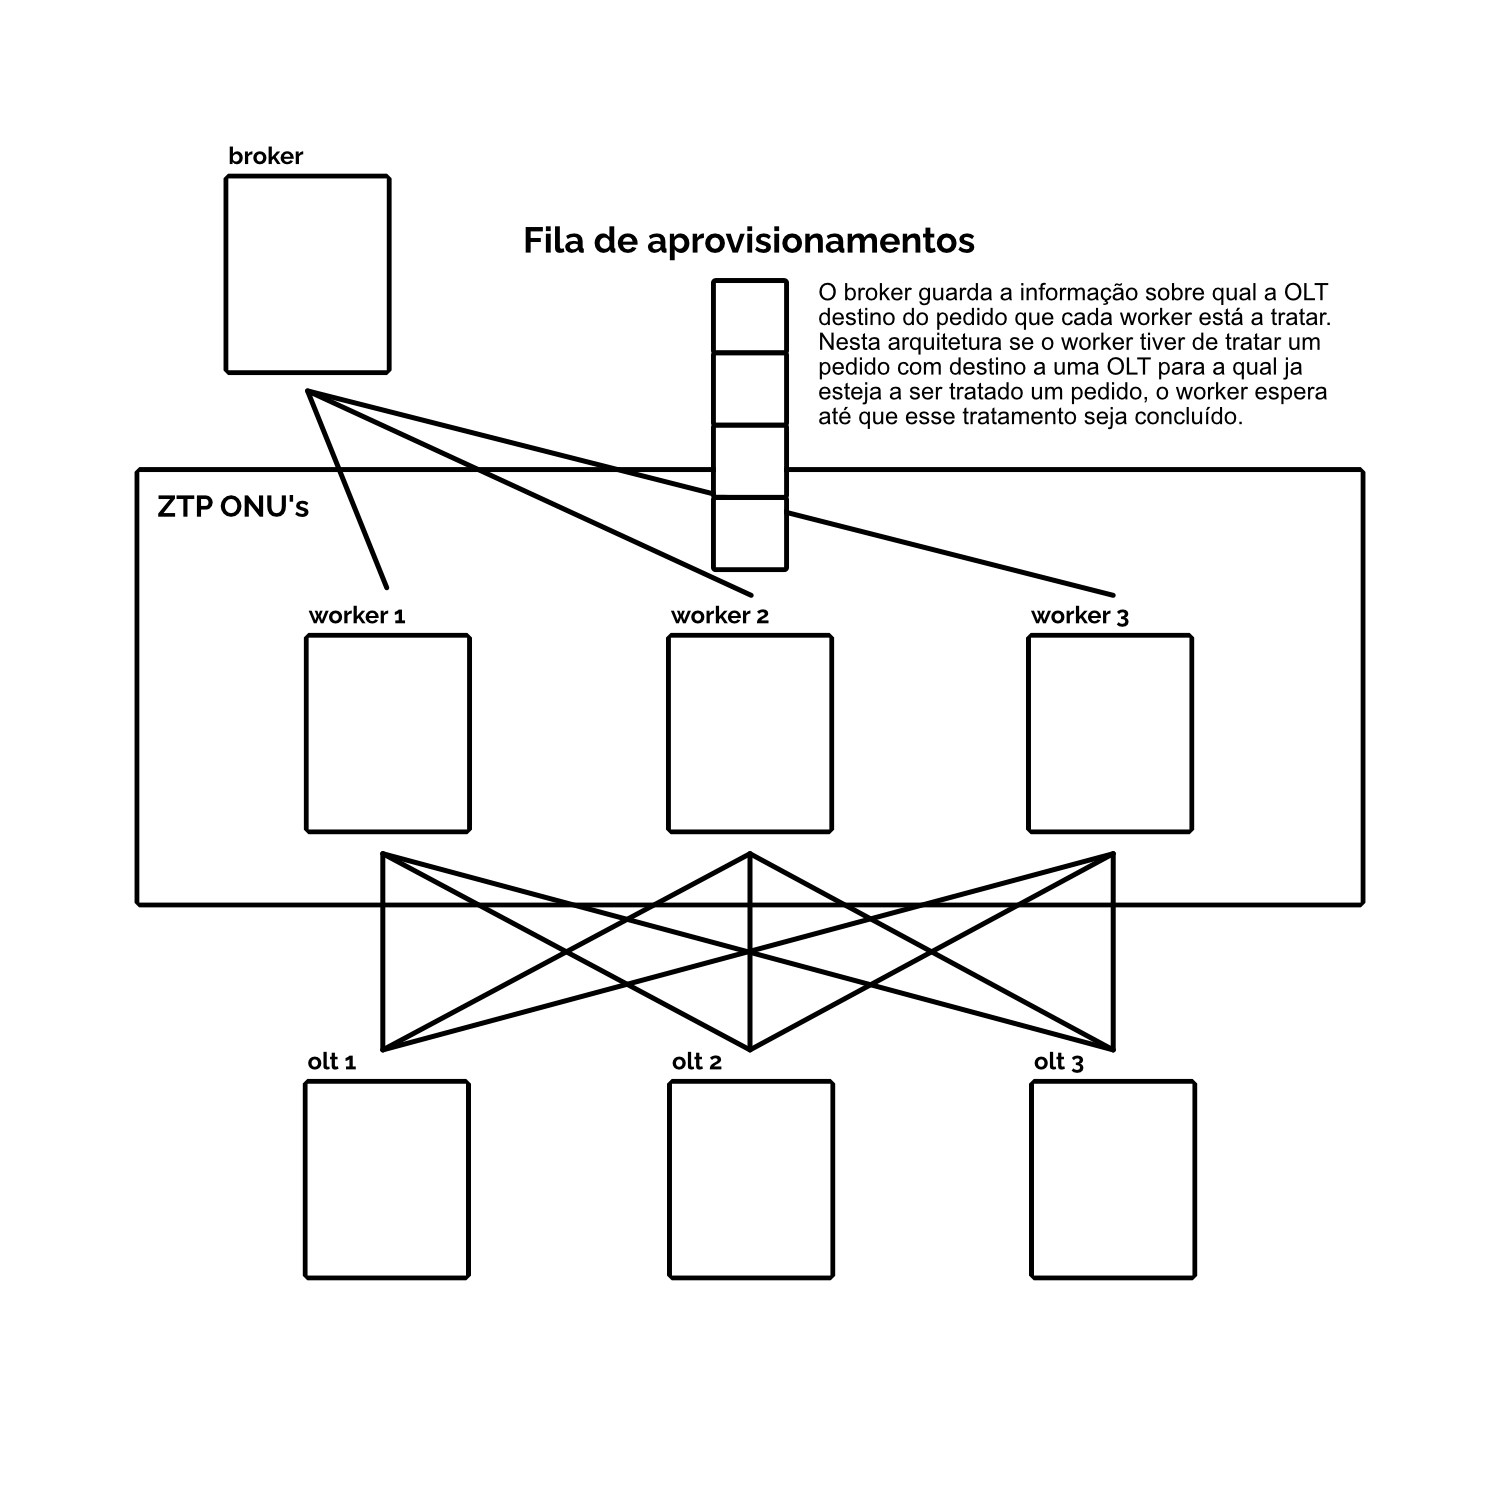
\includegraphics[width=0.8\textwidth]{./assets/gestao_de_filas/arquitetura_algoritmo_2.png}
    \end{figure}    
\end{frame}

\begin{frame}
    \frametitle{Arquitetura melhorada - 2ª alternativa}
    \begin{figure}
        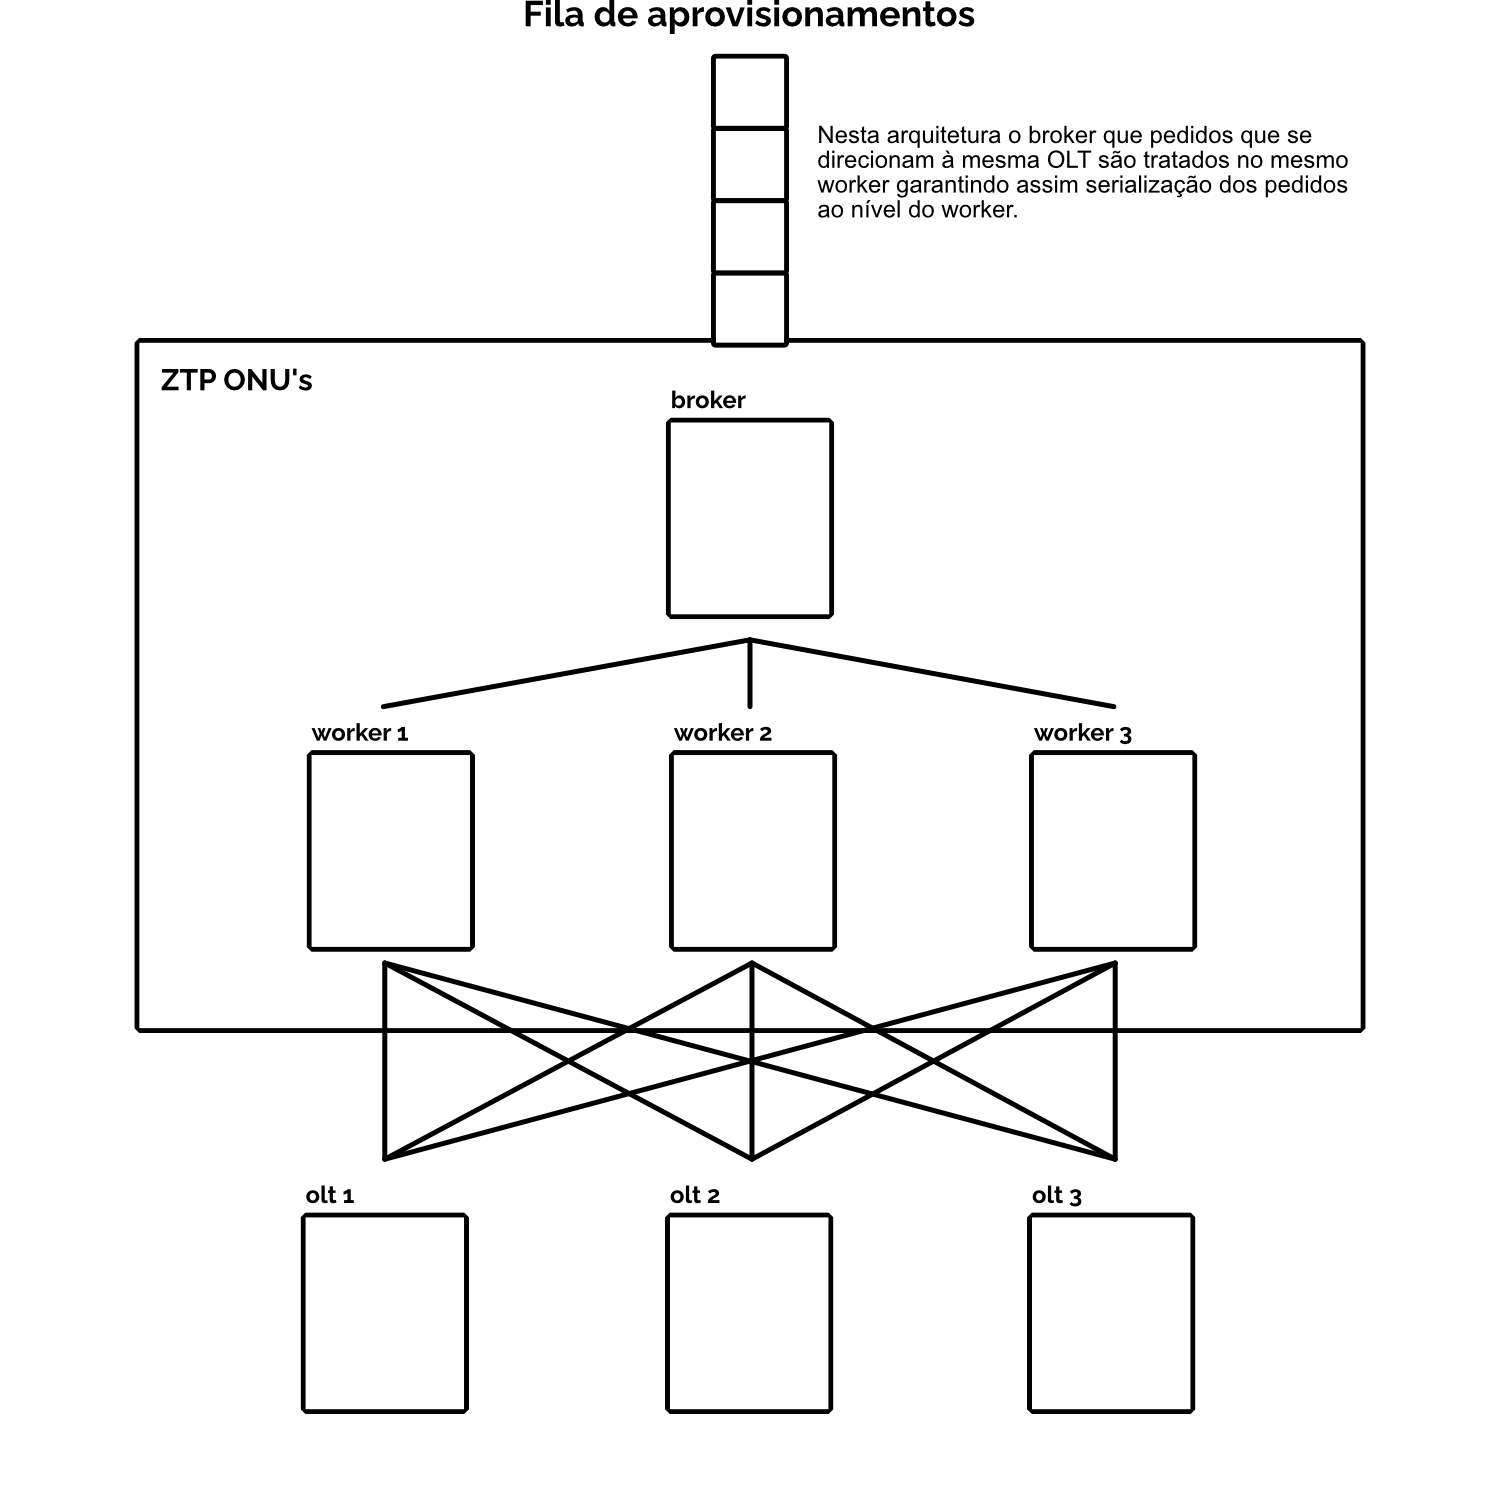
\includegraphics[width=0.7\textwidth]{./assets/gestao_de_filas/arquitetura_algoritmo_3.png}
    \end{figure}    
\end{frame}

\begin{frame}
    \frametitle{Arquitetura melhorada - 3ª alternativa}
    \begin{figure}
        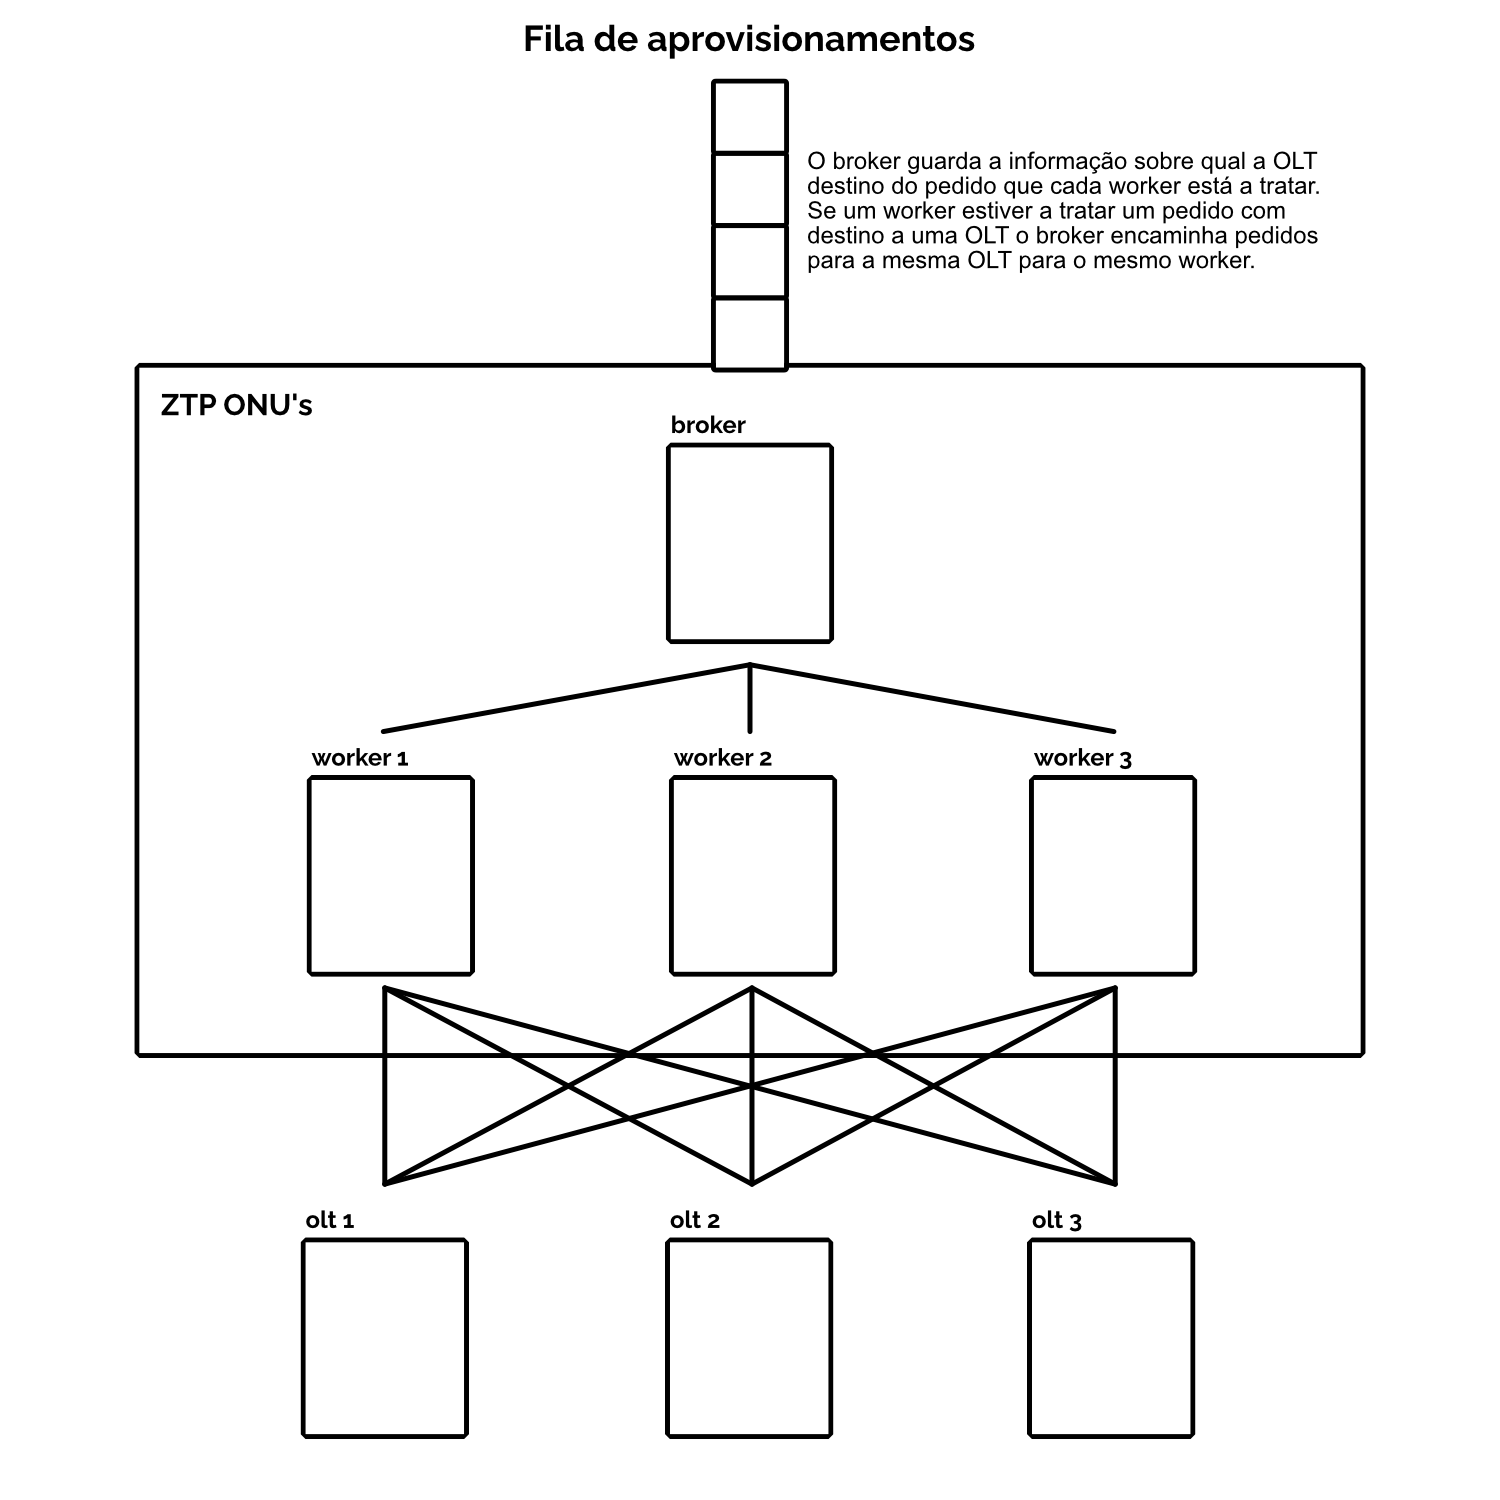
\includegraphics[width=0.7\textwidth]{./assets/gestao_de_filas/arquitetura_algoritmo_4.png}
    \end{figure}
\end{frame}

\begin{frame}
    \frametitle{Ambiente de simulação}
    \begin{itemize}
      \item Fornece um método de comparação objetivo entre as propostas de arquitetura apresentadas.
      \item As métricas que determinam a comparação entre as alternativas são:
      \begin{itemize}
        \item Tempo total de simulação
        \item Número de \textit{timeouts} ocorridos.
      \end{itemize}  
    \end{itemize}  
\end{frame}  

% explicar os ensais que foram feitos e em que condições
\begin{frame}
    \frametitle{Tempo total de simulação em função do número de \textit{workers} (em \textit{ms})}
    \begin{figure}
        \small
        \centering
          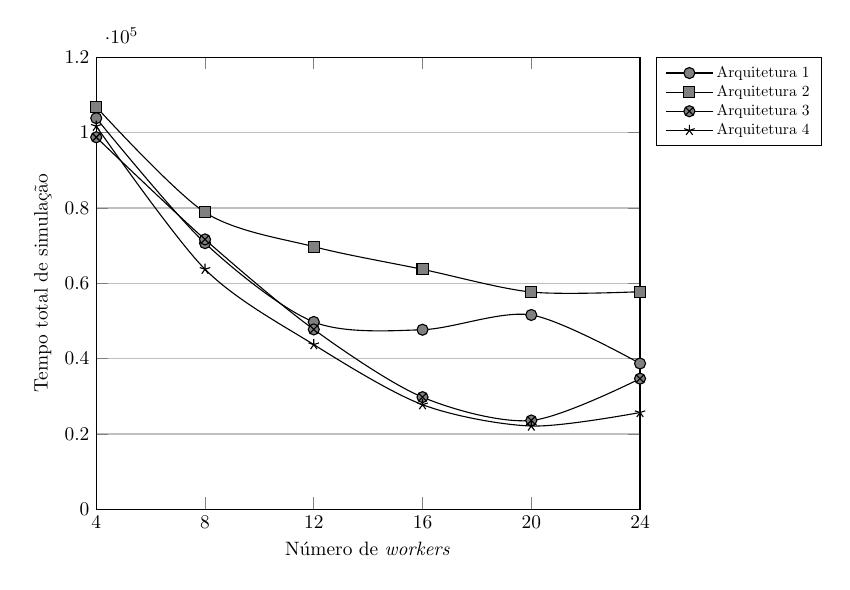
\begin{tikzpicture}
            \begin{axis}[
              style={
                nodes={
                  scale=0.7,
                  transform shape
                }
              },
              xlabel={Número de \textit{workers}},
              ylabel={Tempo total de simulação},
              xmin=4, xmax=24,
              ymin=0, ymax=120000,
              xtick={4, 8, 12, 16, 20, 24},
              ytick={0, 20000, 40000, 60000, 80000, 100000, 120000},
              legend style={ 
                nodes={
                  scale=0.8,
                  transform shape
                },
                at={(1.03, 1)},
                scale=0.05,
                anchor=north west,
                align=left
              },
              cycle list name=black white,
              ymajorgrids=true,
              smooth,
              width=0.7\textwidth
            ]
      
              \addplot coordinates {
                (4, 103859)(8, 70675)(12, 49744)(16, 47681)(20, 51600)(24, 38715)
              };
              \addlegendentry{Arquitetura 1};
      
              \addplot coordinates {
                (4, 106842)(8, 78839)(12, 69734)(16, 63716)(20, 57688)(24, 57778)
              };
              \addlegendentry{Arquitetura 2};
      
              \addplot coordinates {
                (4, 98788)(8, 71665)(12, 47759)(16, 29772)(20, 23578)(24, 34685)
              };
              \addlegendentry{Arquitetura 3};
      
              \addplot coordinates {
                (4, 101725)(8, 63743)(12, 43731)(16, 27771)(20, 22112)(24, 25698)
              };
              \addlegendentry{Arquitetura 4};
      
            \end{axis}
          \end{tikzpicture}
        \caption{Comparação do tempo total da simulação em função do número de \textit{workers}}
      \end{figure}
\end{frame}    

\begin{frame}
    \frametitle{\textit{Timeouts} ocorridos em função do número de \textit{workers}}
    \begin{figure}
        \centering
            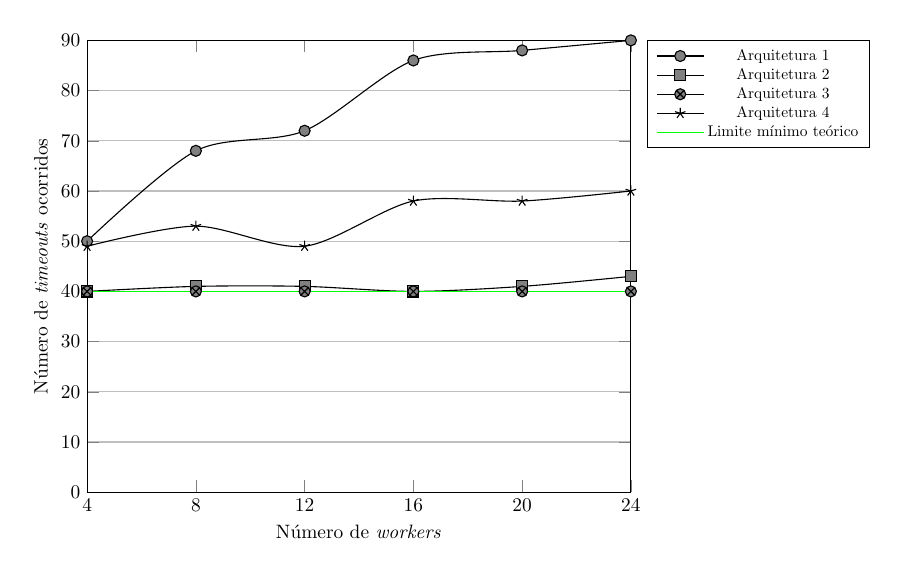
\begin{tikzpicture}
      \begin{axis}[
        style={
          nodes={
            scale=0.7,
            transform shape
          }
        },
        xlabel={Número de \textit{workers}},
        ylabel={Número de \textit{timeouts} ocorridos},
        xmin=4, xmax=24,
        ymin=0, ymax=90,
        xtick={4, 8, 12, 16, 20, 24},
        ytick={0, 10, 20, 30, 40, 50, 60, 70, 80, 90},
        legend style={
          nodes={
            scale=0.8,
            transform shape
          },
          at={(1.03, 1)},
          scale=0.05,
          anchor=north west,
          align=left
        },
        cycle list name=black white,
        ymajorgrids=true,
        smooth,
        width=0.7\textwidth
      ]
  
        \addplot coordinates {
          (4, 50)(8, 68)(12, 72)(16, 86)(20, 88)(24, 90)
        };
        \addlegendentry{Arquitetura 1};
  
        \addplot coordinates {
          (4, 40)(8, 41)(12, 41)(16, 40)(20, 41)(24, 43)
        };
        \addlegendentry{Arquitetura 2};
  
        \addplot coordinates {
          (4, 40)(8, 40)(12, 40)(16, 40)(20, 40)(24, 40)
        };
        \addlegendentry{Arquitetura 3};
  
        \addplot coordinates {
          (4, 49)(8, 53)(12, 49)(16, 58)(20, 58)(24, 60)
        };
        \addlegendentry{Arquitetura 4};
  
        \addplot[green] coordinates {
          (4, 40)(8, 40)(12, 40)(16, 40)(20, 40)(24, 40)
        };
        \addlegendentry{Limite mínimo teórico};
  
      \end{axis}
    \end{tikzpicture}
    \caption{\textit{Timeouts} ocorridos em função do número de \textit{workers}}
  \end{figure}
\end{frame}

\begin{frame}
    \frametitle{Tipos e sequências de mensagens emuladas}
    \textbf{Sequência de mensagens do tipo 1}
    \begin{itemize}
      \item 100\% mensagens do tipo 1
    \end{itemize}  
    \textbf{Sequência de mensagens do tipo 2}
    \begin{itemize}
      \item 10\% mensagens do tipo 2 + 90\% mensagens do tipo 1
    \end{itemize}  
    \textbf{Sequência de mensagens do tipo 3}
    \begin{itemize}
      \item 10\% mensagens do tipo 3 + 10\% mensagens do tipo 2 + 80\% mensagens do tipo 1
    \end{itemize}
    \textit{Tipos de mensagens}
    \begin{itemize}
      \item \textbf{Tipo 1:} \texttt{t} << \texttt{timeout}
      \item \textbf{Tipo 2:} \texttt{t} \textless  \texttt{timeout}
      \item \textbf{Tipo 3:} \texttt{t} >> \texttt{timeout}
    \end{itemize}  
\end{frame}    
